\documentclass[a4paper,11pt,notitlepage]{article}
\usepackage[utf8]{inputenc}	% latin2 - kodowanie iso-8859-2; cp1250 - kodowanie windows
\usepackage[T1]{fontenc}
\usepackage[polish]{babel}
\usepackage[MeX]{polski}
\usepackage[pdftex]{graphicx}
\selectlanguage{polish}

\usepackage{graphicx}

\hyphenation{FreeBSD}

\author{Rafał Rutyna \\ Piotr Pyśk \\ GR3}
\title{Laboratorium Sieci Komputerowych \\ {\small Interfejsy sieciowe}}
\date{\today}

\linespread{1.3}

\usepackage{indentfirst}

\begin{document}
\maketitle
\newpage
\tableofcontents
\newpage

\section{Wstęp}

\section{Program Wi-Fi Analyzer}

Za pomocą programu Wi-Fi Analyzer przeskanowaliśmy eter w budynku Starej 
Kotłowni w poszukiwaniu sieci ZETiIS i pwwifi-students.
Wyniki przedstawia rysunek~\ref{wifi-analyzer}.

\begin{figure}[htb]
  \centering
  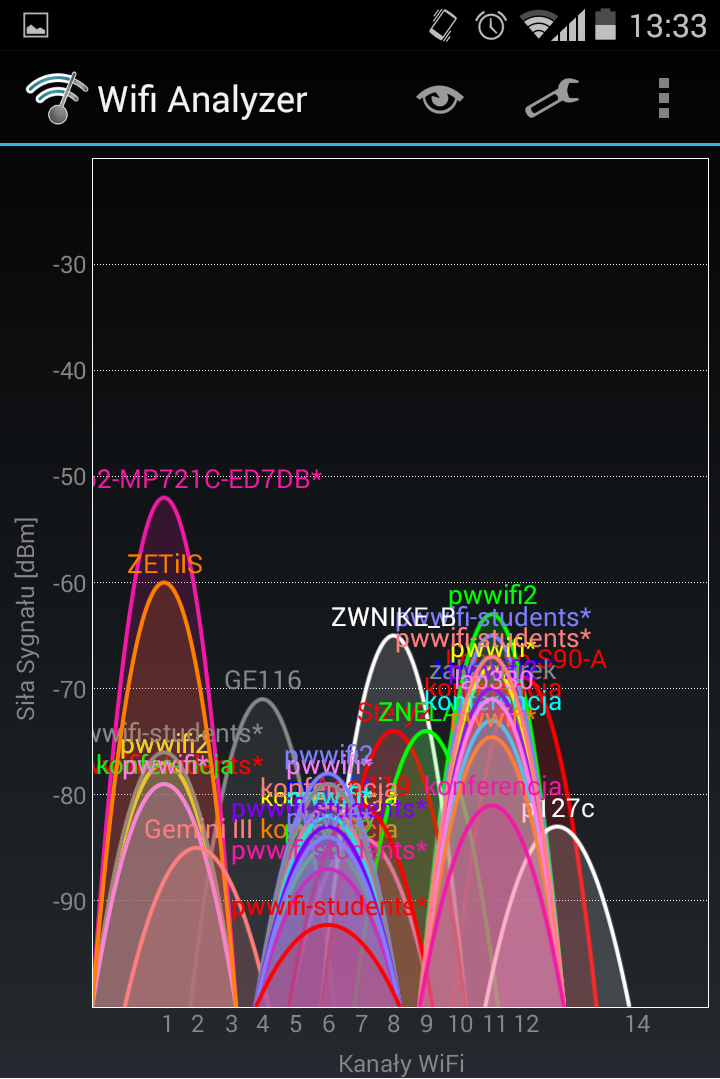
\includegraphics[width=0.5\textwidth]{analyzer.png}
  \caption{Wyniki programu Wifi-Analyzer}
  \label{wifi-analyzer}
\end{figure}

Udało nam się również połączyć z siecią ZETiIS za pomocą telefonu z systemem Android.

\section{Podłącznie interfejsów bezprzewodowych w systemie FreeBSD}

\subsection{Kreacja interfejsu wlan0}

Do stworzenia interefejsu bezprzewodowego na maszynie k5 posłużyliśmy się skryptem 
\begin{verbatim}
 k5% sterowniki -w
\end{verbatim}
Załadowaliśmy sterowniki karty 
\begin{verbatim}
 k5% sudo kldload if_iwn
 k5% sudo kldload wlan_amrr
\end{verbatim}
Następnie wykreowaliśmy interfejs wirtualny
\begin{verbatim}
 k5% wlan=$(sudo ifconfig wlan create wlandev iwn0)
 k5% sudo ifconfig $wlan country PL
 k5% sudo ifconfig $wlan up
\end{verbatim}
W efekcie otrzymaliśmy podniesiony interfejs \verb+wlan0+, który automatycznie podłączył się do sieci \verb+pwwifi+.

\subsection{Połącznie z siecią pwwifi-students}

Przeskanowaliśmy eter w poszukiwaniu sieci \verb+pwwifi-students+.
\begin{verbatim}
 k5% ifconfig wlan0 list scan | grep pwifi-s
pwwifi-stud...  00:24:14:31:37:72    1   54M -88:-95  102 ES   HTCAP WME
pwwifi-stud...  00:24:14:31:95:02    1   54M -85:-95  102 ES   HTCAP WME
pwwifi-stud...  0c:85:25:f2:96:62    1   54M -89:-95  102 ES   HTCAP WME
pwwifi-stud...  00:24:14:31:95:22   11   54M -90:-95  102 ES   HTCAP WME
pwwifi-stud...  00:24:14:31:2f:b2   11   54M -83:-95  102 ES   HTCAP WME
\end{verbatim}
Skorzystaliśmy z gotowego skryptu \verb+pwwifi+. 
\begin{verbatim}
 k5% pwwifi start wlan0
\end{verbatim}
Następnie wpisaliśmy numer albumu i hasło. Sprawdziliśmy połącznie programem \verb+traceroute+.
\begin{verbatim}
 k5% traceroute wp.pl
traceroute: Warning: wp.pl has multiple addresses; using 212.77.98.9
traceroute to wp.pl (212.77.98.9), 64 hops max, 52 byte packets
 1  dns.pwifi-studets.pw.edu.pl (10.68.0.1)  34.522 ms  8.813 ms  23.242 ms
 2  coi-smolna.rtr.pw.edu.pl (194.29.130.1)  6.752 ms  7.757 ms  10.008 ms
 3  c7304.rtr.pw.edu.pl (194.29.132.161)  26.561 ms  4.265 ms  15.967 ms
 4  wp.tpix.pl (195.149.232.110)  19.024 ms  14.834 ms  18.221 ms
 5  rtr4.rtr-int-1.adm.wp-sa.pl (212.77.96.73)  15.040 ms  13.959 ms  13.861 ms
 6  www.wp.pl (212.77.98.9)  13.929 ms  14.180 ms  13.397 ms
\end{verbatim}
Na koniec zakończyliśmy połącznie poleceniem
\begin{verbatim}
 k5% pwwifi stop
\end{verbatim}

\subsection{Połącznie z siecią ZETiIS}


\section{Połącznie równy z równym}
Aby zrealizować ćwiczenie stworzyliśmy interfejs wirtualny, odpowiednio na trasowniku \verb+t5+ oraz \verb+t6+, następnie przypisaliśmy im identyfikator sieci o nazwie 'TEST'. Polecenie wyglądało tak samo dla obu trasowników
\begin{verbatim}
  # ifconfig wlan0 create wlandev ath0 wlanmode adhoc
  # ifconfig wlan0 ssid 'TEST'
\end{verbatim}
Kolejnym krokiem było przypisanie im odpowiednich adresów, dla \verb+t5 +  
\begin{verbatim}
 t5% # ifconfig wlan0 inet 10.1
\end{verbatim}
oraz \verb+t6+:
\begin{verbatim}
 t6 # ifconfig wlan0 inet 10.2
\end{verbatim}
Poprawność naszych działań sprawdziliśmy za pomocą programu ping oraz tcpdump.
\begin{verbatim}
 t5% ping -c 2 10.0.0.2
 PING 10.0.0.2 (10.0.0.2): 56 data bytes

 64 bytes from 10.0.0.2: icmp_seq=0 ttl=64 time=19.418 ms
 64 bytes from 10.0.0.2: icmp_seq=1 ttl=64 time=0.481 ms
 --- 10.0.0.2 ping statistics ---

 2 packets transmitted, 2 packets received, 0.0% packet loss
 round-trip min/avg/max/stddev = 0.481/9.950/19.418/9.468 ms
\end{verbatim}
na maszynie \verb+t6+:
\begin{verbatim}
 t6% # tcpdump -i wlan0
 listening on wlan0, link-type EN10MB (Ethernet), capture size 65535 bytes
 21:08:27.152631 ARP, Request who-has 10.0.0.2 tell 10.0.0.1, length 28
 21:08:27.156381 IP 10.0.0.1 > 10.0.0.2: ICMP echo request, id 14342, seq 0, length 64
 21:08:27.156407 IP 10.0.0.2 > 10.0.0.1: ICMP echo reply, id 14342, seq 0, length 64
 21:08:28.152844 IP 10.0.0.1 > 10.0.0.2: ICMP echo request, id 14342, seq 1, length 64
 21:08:28.152878 IP 10.0.0.2 > 10.0.0.1: ICMP echo reply, id 14342, seq 1, length 64
 6 packets captured
 6 packets received by filter
 0 packets dropped by kernel
\end{verbatim}



\section{Sieć bluetooth} 

Zadaniem było połączyć dwa trasowniki przez interfes bluetooth w profilu czujnika zbliżeniowego.

Na samym początku załadowaliśmy sterowniki USB.
\begin{verbatim}
 t5% # kldload uhci
 t5% # kldload ehci
 t5% # kldload xhci
\end{verbatim}
Drugi w kolejności był stos bluetooth.
\begin{verbatim}
 t5% # kldload ng_ubt
 t5% # service bluetooth start ubt0
\end{verbatim}
Obie czynności wykonaliśmy na trasownikach t5 i t4.

Przeskanowaliśmy eter w poszukiwaniu urządzeń bluetooth.
\begin{verbatim}
 t5% bt -scan

skanuje eter bluetooth ...
00:06:66:00:e3:da	F9	# FireFly RS-232 SPP 	t9
00:06:66:00:e2:84       FB	# FireFly RS-232 SPP 	tb
00:06:66:00:e1:35	FC	# FireFly RS-232 SPP	tc
00:11:67:bc:4d:81	K0	# k0 +	Grzybek 1
00:0c:41:e1:d7:8b	K7	# k7 +
00:15:83:07:51:80	K9	# k9 +	Class 1 Tracer
00:0d:93:1c:47:45	MB	# MacMini (mb = m11)
00:15:83:07:51:60	T4	# t4 +	Class 1 Tracer
\end{verbatim}

W kolejnym kroku włączyliśmy czujnik zbliżeniowy na trasowniku t5.
W wyniku otrzymaliśmy komunikat
\begin{verbatim}
 t5% # bt-proximity t4
 2BLISKO
 0 0 0 0 0 0 0 0 0 0 0 0 0 0 0 0 0 0 0 0 0
 0
\end{verbatim}

W celu utworzenia sieci PAN wykorzystaliśmy skrypt bt-pan wywoływany na maszynie \verb+t5+, działającej jako serwer poleceniem 
\begin{verbatim}
 t5% # bt-pan -s
\end{verbatim}
następnie skonfigurowaliśmy interfejs:
\begin{verbatim}
 t5% # ifconfig tap0 10.5
 t5% hccontrol read_connection_list
 Remote BD_ADDR    Handle Type Mode Role Encrypt Pending Queue State
 T5                     6  ACL    0 SLAV    NONE       0     0 OPEN
\end{verbatim}
analogiczne działanie zrobiliśmy na maszynie \verb+t2+ działającej jako klient:
\begin{verbatim}
 t2% # bt-pan -c t5
 t2% # ifconfig tap0 10.2
\end{verbatim}
Działanie połączenia sprawdziliśmy programem ping oraz tcpdump.
\begin{verbatim}
 t2% ping -c 2 10.5
PING 10.5 (10.0.0.5): 56 data bytes
64 bytes from 10.0.0.5: icmp_seq=0 ttl=64 time=28.511 ms
64 bytes from 10.0.0.5: icmp_seq=1 ttl=64 time=20.370 ms
\end{verbatim}

\begin{verbatim}
 t5% # tcpdump -i tap0 
tcpdump: verbose output suppressed, use -v or -vv for full protocol decode
listening on tap0, link-type EN10MB (Ethernet), capture size 65535 bytes
21:22:27.615820 ARP, Request who-has 10.0.0.5 tell 10.0.0.2, length 28
21:22:27.615925 ARP, Reply 10.0.0.5 is-at 00:08:1b:00:2e:e3 (oui Unknown), length 28
21:22:27.630737 IP 10.0.0.2 > 10.0.0.5: ICMP echo request, id 13571, seq 0, length 64
21:22:27.630860 IP 10.0.0.5 > 10.0.0.2: ICMP echo reply, id 13571, seq 0, length 64
21:22:28.621617 IP 10.0.0.2 > 10.0.0.5: ICMP echo request, id 13571, seq 1, length 64
21:22:28.621809 IP 10.0.0.5 > 10.0.0.2: ICMP echo reply, id 13571, seq 1, length 64
\end{verbatim}


\section{Wnioski}

\end{document}
